\section{Eigenvalue method with complex eigenvalues}
\label{eigenmethod-cplx:section}

\LAtt{3.4, 3.7}

\LO{
\item Use Euler's formula to find a real-valued general solution to a first order system with complex eigenvalues and
\item Solve initial value problems from all of these cases once the general solution has been found. 
}

As we have seen previously, a matrix may very well have complex eigenvalues even if all the entries are
real. However, this may seem concerning going forward into solutions to differential equations that require these complex numbers in them. We will see in this section that we can still write solutions this way, but we no longer have straight-line solutions.  Take, for example,
\begin{equation*}
{\vec{x}}' = 
\begin{bmatrix}
1 & 1 \\
-1 & 1
\end{bmatrix}
\vec{x} .
\end{equation*}
Let us compute the eigenvalues of
the matrix $P = \left[ \begin{smallmatrix} 1 & 1 \\ -1 & 1 \end{smallmatrix}
\right]$.
\begin{equation*}
\det(P - \lambda I) =
\det\left(
\begin{bmatrix}
1-\lambda & 1 \\
-1 & 1-\lambda
\end{bmatrix}
\right)
= {(1-\lambda)}^2 + 1
= \lambda^2 - 2 \lambda + 2 = 0 .
\end{equation*}
Thus $\lambda = 1 \pm i$.
Corresponding eigenvectors are also complex.
Start with $\lambda = 1-i$.
\begin{align*}
\bigl(P-(1-i) I\bigr) \vec{v} & = \vec{0} , \\
\begin{bmatrix}
i & 1 \\
-1 & i
\end{bmatrix}
\vec{v} = \vec{0}.
\end{align*}
The equations $i v_1 + v_2 = 0$ and $-v_1 + iv_2 = 0$
are multiples of each other. This may be trickier to spot than the real version, but that is because they are \emph{complex} multiples of each other. If we multiply the first equation by $i$, we get exactly the second one. So we only need to consider one of them.
After picking $v_2 = 1$, for example, we have an
eigenvector
$\vec{v} = \left[ \begin{smallmatrix} i \\ 1 \end{smallmatrix} \right]$.
In similar fashion we find that
$\left[ \begin{smallmatrix} -i \\ 1 \end{smallmatrix} \right]$
is an eigenvector corresponding to the eigenvalue $1+i$.

We could write the solution as
\begin{equation*}
\vec{x} =
c_1 \begin{bmatrix} i \\ 1 \end{bmatrix} e^{(1-i)t} +
c_2 \begin{bmatrix} -i \\ 1 \end{bmatrix} e^{(1+i)t}
=
\begin{bmatrix}
c_1 i e^{(1-i)t} - c_2 i e^{(1+i)t} \\
c_1 e^{(1-i)t} + c_2 e^{(1+i)t}
\end{bmatrix} .
\end{equation*}
We would then need to look for complex values $c_1$ and $c_2$ to solve
any initial conditions.  It is perhaps not completely clear
that we get a real solution.  After solving for $c_1$ and $c_2$,
we could use
\hyperref[eulersformula]{Euler's formula} and do the
whole song and dance we did before, but we will not.   We will apply
the formula in a smarter way first to find independent real solutions.

\medskip

In this case, we only needed one of the two eigenvectors to get the general solution, which happens because the complex eigenvalues and eigenvectors always come in conjugate pairs. First a small detour.  The real part of
a complex number $z$ can be computed as $\frac{z + \bar{z}}{2}$, where
the bar above $z$ means $\overline{a+ib} = a -ib$.  This operation is called the
\emph{\myindex{complex conjugate}}.
If $a$ is a real number, then $\bar{a} = a$.
Similarly
we bar whole vectors or matrices by taking the complex conjugate
of every entry.  Suppose a matrix $P$ is real.  Then
$\overline{P} = P$, and so $\overline{P\vec{x}} = \overline{P} \,
\overline{\vec{x}} = P \overline{\vec{x}}$.
Also the complex conjugate of 0 is still 0,
therefore,
\begin{equation*}
\vec{0} = \overline{\vec{0}} = 
\overline{(P-\lambda I)\vec{v}}
=
(P-\bar{\lambda} I)\overline{\vec{v}} .
\end{equation*}
In other words, if $\lambda = a+ib$ is an eigenvalue, then so is $\bar{\lambda} = a-ib$.
And if $\vec{v}$ is an eigenvector corresponding to the eigenvalue
$\lambda$, then $\overline{\vec{v}}$ is an eigenvector corresponding
to the eigenvalue $\bar{\lambda}$.  

Suppose $a + ib$ is a complex eigenvalue of $P$, and $\vec{v}$
is a corresponding eigenvector.  Then
\begin{equation*}
\vec{x}_1 = \vec{v} e^{(a+ib)t}
\end{equation*}
is a solution (complex-valued) of
${\vec{x}}' = P \vec{x}$.  \hyperref[eulersformula]{Euler's formula}
shows that $\overline{e^{a+ib}} =
e^{a-ib}$,
and so
\begin{equation*}
\vec{x}_2 = \overline{\vec{x}_1} = \overline{\vec{v}} e^{(a-ib)t}
\end{equation*}
is also a solution.
As $\vec{x}_1$ and $\vec{x}_2$ are solutions, the function
\begin{equation*}
\vec{x}_3 =
\operatorname{Re} \vec{x}_1 =
\operatorname{Re} \vec{v} e^{(a+ib)t} =
\frac{\vec{x}_1 + \overline{\vec{x}_1}}{2}  =
\frac{\vec{x}_1 + \vec{x}_2}{2} 
=
\frac{1}{2} \vec{x}_1 + \frac{1}{2}\vec{x}_2
\end{equation*}
is also a solution.  And $\vec{x}_3$ is real-valued!  Similarly as
$\operatorname{Im} z = \frac{z-\bar{z}}{2i}$ is the imaginary part, we find
that
\begin{equation*}
\vec{x}_4 =
\operatorname{Im} \vec{x}_1 =
\frac{\vec{x}_1 - \overline{\vec{x}_1}}{2i}  =
\frac{\vec{x}_1 - \vec{x}_2}{2i} .
\end{equation*}
is also a real-valued solution.  It turns out that $\vec{x}_3$ and
$\vec{x}_4$ are linearly independent.
We will use \hyperref[eulersformula]{Euler's formula}
to separate out the real and imaginary part.

\medskip

Returning to our problem,
\begin{equation*}
\vec{x}_1 =
\begin{bmatrix} i \\ 1 \end{bmatrix} e^{(1-i)t}
=
\begin{bmatrix} i \\ 1 \end{bmatrix} \left( e^t \cos t - i e^t \sin t \right)
=
\begin{bmatrix}
i e^t \cos t + e^t \sin t  \\
e^t \cos t - i e^t \sin t
\end{bmatrix}
=
\begin{bmatrix}
e^t \sin t  \\
e^t \cos t
\end{bmatrix}
+ i
\begin{bmatrix}
e^t \cos t  \\
- e^t \sin t
\end{bmatrix}
.
\end{equation*}
Then
\begin{equation*}
\operatorname{Re} \vec{x}_1 = 
\begin{bmatrix}
e^t \sin t  \\
e^t \cos t
\end{bmatrix} ,
\qquad \text{and} \qquad
\operatorname{Im} \vec{x}_1 = 
\begin{bmatrix}
e^t \cos t \\
- e^t \sin t
\end{bmatrix} ,
\end{equation*}
are the two real-valued linearly independent solutions we seek.

\begin{exercise}
Check that these really are solutions.
\end{exercise}

This gives that we can write the general solution to this problem as
\begin{equation*}
\vec{x}
=
c_1
\begin{bmatrix}
e^t \sin t  \\
e^t \cos t
\end{bmatrix} 
+ c_2
\begin{bmatrix}
e^t \cos t \\
-e^t \sin t
\end{bmatrix} 
=
\begin{bmatrix}
c_1 e^t \sin t + c_2 e^t \cos t \\
c_1 e^t \cos t - c_2 e^t \sin t
\end{bmatrix} .
\end{equation*}
This solution is real-valued for real $c_1$ and $c_2$.  We now solve
for any initial conditions we may have. Notice that the $i$ has been dropped from the part of the process where we split the complex solution into real and imaginary parts. The point is that the real and imaginary parts of the solution are independently solutions to the equation, and so we can use them to form our basis of solutions with constants $c_1$ and $c_2$ in front of them. We want everything to be real, and this process allows us to do it.

\medskip

Let us summarize as a theorem. 

\begin{theorem1}{}
Let $P$ be a real-valued constant matrix.
If $P$ has a complex eigenvalue $a+ib$ and a corresponding eigenvector
$\vec{v}$, then $P$ also has a complex eigenvalue $a-ib$ with
a corresponding eigenvector $\overline{\vec{v}}$.
Furthermore,
${\vec{x}}' = P\vec{x}$ has
two linearly independent real-valued solutions
\begin{equation*}
\vec{x}_1 = \operatorname{Re} \vec{v} e^{(a+ib)t} ,
\qquad
\text{and}
\qquad
\vec{x}_2 = \operatorname{Im} \vec{v} e^{(a+ib)t} .
\end{equation*}
\end{theorem1}

The main point here is that the real and imaginary parts of these complex solutions are the real-valued independent solutions that we seek. Compare this to Theorem \ref{thm:realimagparts} in \sectionref{complexroots:section}, where we saw that the same idea worked for second order equation with complex roots.

For each pair of complex eigenvalues $a+ib$ and $a-ib$,
we get two real-valued linearly
independent solutions.
We then go on to the next
eigenvalue, which is either a real eigenvalue or another complex eigenvalue
pair.  If we have $n$ distinct eigenvalues (real or complex), then we end up with $n$ linearly independent solutions.
If we had only two equations ($n=2$) as in the example above,
then once we found two solutions we are
finished, and our general solution is
\begin{equation*}
\vec{x} =
c_1 \vec{x}_1 + c_2 \vec{x}_2
= 
c_1 \bigl( \operatorname{Re} \vec{v} e^{(a+ib)t} \bigr) +
c_2 \bigl( \operatorname{Im} \vec{v} e^{(a+ib)t} \bigr)
.
\end{equation*}

\begin{example}
Find the solution to the initial value problem
\begin{equation*}
\vec{x}' = \begin{bmatrix} 1 & 4 \\ -2 & -3 \end{bmatrix}\vec{x} \qquad \vec{x}(0) = \begin{bmatrix} 1 \\ -2 \end{bmatrix}.
\end{equation*}
\end{example}

\begin{exampleSol}
We start by looking for the eigenvalues and eigenvectors of the coefficient matrix. This results in the polynomial
\begin{equation*}
\det(P - \lambda I) = (1-\lambda)(-3-\lambda) - (4)(-2) = \lambda^2 + 3\lambda - \lambda  - 3 + 8 = \lambda^2 + 2\lambda + 5.
\end{equation*}
This polynomial does not factor, but the quadratic formula gives that the roots are
\begin{equation*}
\lambda = \frac{-2 \pm \sqrt{4 - (4)(1)(5)}}{2} = -1 \pm \frac{\sqrt{-16}}{2} = -1 \pm 2i.
\end{equation*}
Thus, we are in the complex roots case, and can work from there. We need to find the complex eigenvector for one of these eigenvalues and then split into real and imaginary parts to get the general solution. 

For the eigenvalue $\lambda = -1 + 2i$, the matrix equation becomes
\begin{equation*}
(P - \lambda I)\vec{v} = \begin{bmatrix} 1 - (-1 + 2i) & 4 \\ -2 & -3 - (-1 + 2i) \end{bmatrix} \vec{v} = \begin{bmatrix} 2 - 2i & 4 \\ -2 & -2 -2i \end{bmatrix}\vec{v} = \vec{0}. 
\end{equation*}
The two simultaneous equation that we need to solve for the vector $v$ are 
\begin{equation*}
(2-2i)v_1 + 4v_2 = 0 \qquad -2v_1 + (-2-2i)v_2 = 0
\end{equation*}
and these equations don't appear to be redundant. However, this is because they are complex multiples of each other, not just real multiples. To see this, we can multiply the first equation by the complex conjugate of the first coefficient. The idea is that if we do so, this first coefficient will be real, and then we can compare it to the second equation. If we multiply the first equation by $2 + 2i$, since $(2+2i)(2-2i) = 8$, it becomes
\begin{equation*}
8v_1 + 4(2+2i)v_2 = 0
\end{equation*}
and this is $-4$ times the second equation above. Therefore, they are redundant, and we can just pick one of them in order to find possible values of $v_1$ and $v_2$. If we divide this newest equation by $8$, it becomes
\begin{equation*}
v_1 + (1+i)v_2 = 0.
\end{equation*}
Based on this equation, we can pick $v_2 = -1$ and $v_1 = 1+i$. Therefore, the eigenvector for $\lambda = -1 + 2i$ is $\left[ \begin{smallmatrix} 1+i \\ -1 \end{smallmatrix} \right]$. This means that a complex-valued solution to this differential equation is
\begin{equation*}
\vec{x}(t) = \begin{bmatrix} 1+i \\ -1 \end{bmatrix} e^{(-1 + 2i)t}.
\end{equation*}

Now, we want to split this solution into real and imaginary parts in order to get a real-valued general solution. We apply Euler's formula to do so:
\begin{equation*}
\begin{split}
\vec{x}(t) &= \begin{bmatrix} 1+i \\ -1 \end{bmatrix} e^{(-1 + 2i)t} \\
&= \begin{bmatrix} 1+i \\ -1 \end{bmatrix} e^{-t}(\cos(2t) + i\sin(2t)) \\
&= e^{-t} \begin{bmatrix} \cos(2t) + i\sin(2t)+i\cos(2t) - \sin(2t) \\ -\cos(2t) - i\sin(2t)  \end{bmatrix} \\
&= \begin{bmatrix} e^{-t}\cos(2t) - e^{-t}\sin(2t) \\ -e^{-t}\cos(2t)\end{bmatrix} + i\begin{bmatrix} e^{-t}\sin(2t) + e^{-t}\cos(2t) \\ -e^{-t}\sin(2t) \end{bmatrix}.
\end{split}
\end{equation*}
Therefore, we can take the real and imaginary parts of this solution to get a general solution as
\begin{equation*}
\vec{x}(t) = c_1 \begin{bmatrix} e^{-t}\cos(2t) - e^{-t}\sin(2t) \\ -e^{-t}\cos(2t)\end{bmatrix} +  c_2\begin{bmatrix} e^{-t}\sin(2t) + e^{-t}\cos(2t) \\ -e^{-t}\sin(2t) \end{bmatrix}.
\end{equation*}

\begin{exercise}
Work out the eigenvector and general solution from eigenvalue $\lambda = -1 - 2i$ and verify that it is an equivalent general solution to the one above.
\end{exercise}

Finally, we need to solve the initial value problem. Plugging in $t=0$ gives 
\begin{equation*}
\vec{x}(0) = c_1 \begin{bmatrix} 1 \\ -1 \end{bmatrix} + c_2 \begin{bmatrix} 1 \\ 0 \end{bmatrix} = \begin{bmatrix} 1 \\ -2 \end{bmatrix}.
\end{equation*}

The two equations that we get from here is $c_1 + c_2 = 1$ and $-c_1 = -2$, so that $c_1 = 2$ and $c_2 = -1$. Therefore, the solution to the initial value problem is
\begin{equation*}
\vec{x}(t) = 2\begin{bmatrix} e^{-t}\cos(2t) - e^{-t}\sin(2t) \\ -e^{-t}\cos(2t)\end{bmatrix} - \begin{bmatrix} e^{-t}\sin(2t) + e^{-t}\cos(2t) \\ -e^{-t}\sin(2t) \end{bmatrix} = \begin{bmatrix} 2e^{-t}\cos(2t) - 3e^{-t}\sin(2t) \\ -2e^{-t}\cos(2t) + e^{-t}\sin(2t) \end{bmatrix}.
\end{equation*}
\end{exampleSol}

\subsection{Phase Portraits}

Similarly to the real eigenvalue situation, we have three different cases for the phase portrait when the eigenvalues of a 2x2 matrix are complex. As metioned before, our basis solutions that we are using to form the general solution are no longer just exponential terms. They involve sines and cosines, and so are not straight lines anymore. Therefore, these solutions will not have straight lines in them, but we can still uses these basis solutions to help determine and describe the overall behavior of the solutions to the system for a variety of initial conditions. 

\emph{Case 1.} Suppose the eigenvalues are purely imaginary.
That is, suppose the eigenvalues are $\pm ib$.  For example,
let $P = 
\left[ \begin{smallmatrix} 0 & 1 \\ -4 & 0 \end{smallmatrix} \right]$.
The eigenvalues turn out to be $\pm 2i$ and eigenvectors are
$\left[ \begin{smallmatrix} 1 \\ 2i \end{smallmatrix} \right]$ and
$\left[ \begin{smallmatrix} 1 \\ -2i \end{smallmatrix} \right]$.  Consider
the eigenvalue $2i$ and its eigenvector
$\left[ \begin{smallmatrix} 1 \\ 2i \end{smallmatrix} \right]$.
The real and imaginary
parts of $\vec{v} e^{2it}$ are
\begin{equation*}
\operatorname{Re} \left(
\begin{bmatrix} 1 \\ 2i \end{bmatrix} e^{2it}\right) =
\begin{bmatrix} \cos (2t) \\ -2 \sin (2t)  \end{bmatrix} ,
\qquad
\operatorname{Im} \left(
\begin{bmatrix} 1 \\ 2i \end{bmatrix} e^{2it}\right) =
\begin{bmatrix} \sin (2t) \\ 2 \cos (2t) \end{bmatrix} .
\end{equation*}
We can take any linear combination of them to get other solutions,
which one we take
depends on the initial
conditions.  Now note that the real part is
a parametric equation for an ellipse.  Same with the imaginary part
and in fact any linear combination of the two.
This is what happens in general when the eigenvalues are purely imaginary.
So when the eigenvalues are purely imaginary, we get
\emph{ellipses\index{ellipses (vector field)}} for the
solutions.  This type of picture is sometimes called a
\emph{\myindex{center}}.  See \figurevref{pln:ellipsesfig}.

\begin{myfig}
\parbox[t]{3.0in}{
 \capstart
 \diffyincludegraphics{width=3in}{width=4.5in}{pln-ellipses}
 \caption{Example center vector field.\label{pln:ellipsesfig}}
}
\quad
\parbox[t]{3.0in}{
 \capstart
 \diffyincludegraphics{width=3in}{width=4.5in}{pln-spiral-source}
 \caption{Example spiral source vector field.\label{pln:spiral-sourcefig}}
}
\end{myfig}

\medskip

\emph{Case 2.} Now suppose the complex eigenvalues have a positive real
part.  That is, suppose the eigenvalues are $a \pm ib$ for some $a > 0$.
For example, let $P = 
\left[ \begin{smallmatrix} 1 & 1 \\ -4 & 1 \end{smallmatrix} \right]$.
The eigenvalues turn out to be $1\pm 2i$ and eigenvectors are
$\left[ \begin{smallmatrix} 1 \\ 2i \end{smallmatrix} \right]$ and
$\left[ \begin{smallmatrix} 1 \\ -2i \end{smallmatrix} \right]$.  We take
$1 + 2i$ and its eigenvector
$\left[ \begin{smallmatrix} 1 \\ 2i \end{smallmatrix} \right]$ and find
the real and imaginary parts of
$\vec{v} e^{(1+2i)t}$ are
\begin{equation*}
\operatorname{Re}\left(
\begin{bmatrix} 1 \\ 2i \end{bmatrix} e^{(1+2i)t}\right) =
e^t
\begin{bmatrix} \cos (2t) \\ -2 \sin (2t)  \end{bmatrix} ,
\qquad
\operatorname{Im}\left(
\begin{bmatrix} 1 \\ 2i \end{bmatrix} e^{(1+2i)t} \right)=
e^t
\begin{bmatrix} \sin (2t) \\ 2 \cos (2t) \end{bmatrix} .
\end{equation*}
Note the $e^t$ in front of the solutions.  The solutions
grow in magnitude while spinning around the origin.  Hence we get
a \emph{\myindex{spiral source}}.
See \figurevref{pln:spiral-sourcefig}.

\medskip

\emph{Case 3.} Finally suppose the complex eigenvalues have a negative real
part.  That is, suppose the eigenvalues are $-a \pm ib$ for some $a > 0$.
For example, let $P = 
\left[ \begin{smallmatrix} -1 & -1 \\ 4 & -1 \end{smallmatrix} \right]$.
The eigenvalues turn out to be $-1\pm 2i$ and eigenvectors are
$\left[ \begin{smallmatrix} 1 \\ -2i \end{smallmatrix} \right]$ and
$\left[ \begin{smallmatrix} 1 \\ 2i \end{smallmatrix} \right]$.  We take
$-1 - 2i$ and its eigenvector
$\left[ \begin{smallmatrix} 1 \\ 2i \end{smallmatrix} \right]$ and find
the real and imaginary parts of
$\vec{v} e^{(-1-2i)t}$ are
\begin{equation*}
\operatorname{Re}\left(
\begin{bmatrix} 1 \\ 2i \end{bmatrix} e^{(-1-2i)t}\right) =
e^{-t}
\begin{bmatrix} \cos (2t) \\ 2 \sin (2t)  \end{bmatrix} ,
\qquad
\operatorname{Im}\left(
\begin{bmatrix} 1 \\ 2i \end{bmatrix} e^{(-1-2i)t}\right) =
e^{-t}
\begin{bmatrix} -\sin (2t) \\ 2 \cos (2t) \end{bmatrix} .
\end{equation*}
Note the $e^{-t}$ in front of the solutions.  The solutions
shrink in magnitude while spinning around the origin.  Hence we get
a \emph{\myindex{spiral sink}}.
See \figurevref{pln:spiral-sinkfig}.

\begin{myfig}
\capstart
\diffyincludegraphics{width=2.8in}{width=4.5in}{pln-spiral-sink}
\caption{Example spiral sink vector field.\label{pln:spiral-sinkfig}}
\end{myfig}


\subsection{Exercises}


\begin{exercise}
Find the general solution of $x_1' = x_1 -2 x_2$,
$x_2' = 2 x_1 + x_2$ using the eigenvalue method.
Do not use complex exponentials in your solution.
\end{exercise}
\comboSol{%
}
{%
$C_1e^t\left[\begin{smallmatrix} -\sin(2t)\\ \cos(2t) \end{smallmatrix}\right] + C_2e^{t}\left[\begin{smallmatrix} \cos(2t) \\ \sin(2t) \end{smallmatrix}\right]$ \hfill\raisebox{-0.5\height}{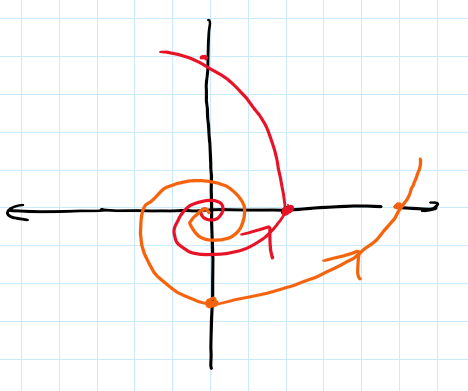
\includegraphics[height=1.5in]{Images/phaseportrait_1_n2_2_1_sketch.png}}\hfill\hfill
}

\begin{exercise}\ansMark%
Solve $x_1' = x_2$, $x_2' = -x_1$ using the eigenvalue method.
\end{exercise}
\exsol{%
$\vec{x} =
C_1 \left[ \begin{smallmatrix}
\cos(t) \\ -\sin(t)
\end{smallmatrix}\right]
+
C_2 \left[ \begin{smallmatrix}
\sin(t) \\ \cos(t)
\end{smallmatrix}\right]$ \hfill\raisebox{-0.5\height}{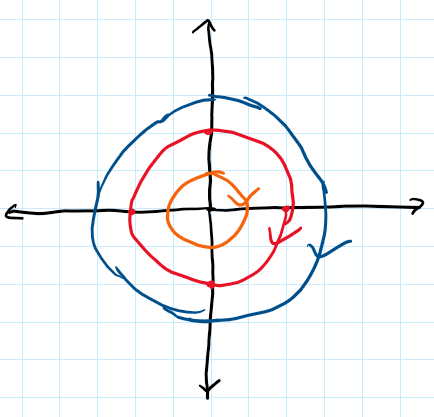
\includegraphics[height=1.5in]{Images/phaseportrait_0_1_n1_0_sketch.png}}\hfill\hfill
}

\begin{exercise}
A $2\times 2$ matrix $A$ has complex eigenvector $\displaystyle \vec{v}=\begin{bmatrix} 1\\ i \end{bmatrix}$ corresponding to eigenvalue $\lambda=-1+3i$. %4.5
\begin{tasks}
\task Use Euler's Formula to find the (real-valued) general solution to the system $\vec{x}'=A\vec{x}$.
\task Sketch the phase portrait of this system.
\end{tasks}
\end{exercise}
\comboSol{%
}
{%
$\vec{x}(t) = C_1e^{-t}\left[\begin{smallmatrix} \cos(3t)\\ -\sin(3t) \end{smallmatrix}\right] + C)2e^{-t}\left[\begin{smallmatrix} \sin(3t)\\ \cos(3t) \end{smallmatrix}\right]$  \hfill\raisebox{-0.5\height}{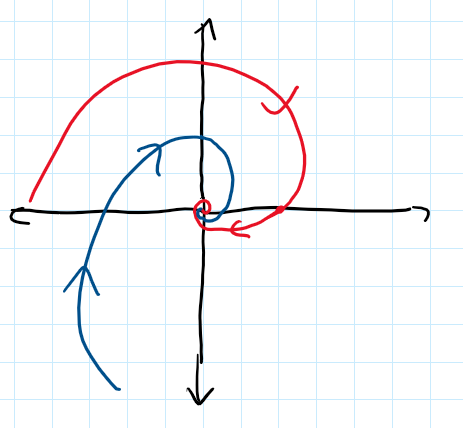
\includegraphics[height=1.5in]{Images/phaseportrait_sketch_fromevec_complex.png}}\hfill\hfill
}

\begin{exercise}\ansMark%
\leavevmode
\begin{tasks}
\task
Compute eigenvalues and eigenvectors of
$A=\left[ \begin{smallmatrix}
1 & 1 \\
-1 & 0 
\end{smallmatrix}\right]$.
\task
Solve the system $\vec{x}\,' = A\vec{x}$.
\task 
Sketch the phase portrait for this system
\end{tasks}
\end{exercise}
\exsol{%
a)
Eigenvalues: $\frac{1+\sqrt{3}i}{2},
\frac{1-\sqrt{3}i}{2}$,
\quad
Eigenvectors:
$\left[ \begin{smallmatrix}
-2 \\ 1-\sqrt{3}i
\end{smallmatrix}\right]$,
$\left[ \begin{smallmatrix}
-2 \\ 1+\sqrt{3}i
\end{smallmatrix}\right]$
\\
b)
$\vec{x} = C_1
e^{t/2}
\left[ \begin{smallmatrix}
-2\cos\bigl(\frac{\sqrt{3}t}{2}\bigr)
\\
\cos\bigl(\frac{\sqrt{3}t}{2}\bigr) + \sqrt{3}\sin\bigl(\frac{\sqrt{3}t}{2}\bigr)
\end{smallmatrix}\right]
+
C_2
e^{t/2}
\left[ \begin{smallmatrix}
- 2\sin\bigl(\frac{\sqrt{3}t}{2}\bigr)
\\
\sin\bigl(\frac{\sqrt{3}t}{2}\bigr) -\sqrt{3}\cos\bigl(\frac{\sqrt{3}t}{2}\bigr)
\end{smallmatrix}\right]$ \quad c)~ \hfill\raisebox{-0.5\height}{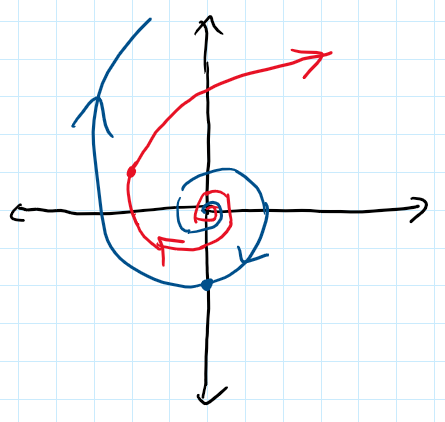
\includegraphics[height=1.5in]{Images/phaseportrait_1_1_n1_0_sketch.png}}\hfill\hfill
}

\begin{exercise}
Consider the system
\begin{equation*}
\begin{bmatrix} x' \\ y' \end{bmatrix} = \begin{bmatrix} 1& -2 \\ 5 & -1 \end{bmatrix} \begin{bmatrix} x \\ y \end{bmatrix}.
\end{equation*} %4.5
\begin{tasks}
\task Find the general solution.
\task Sketch the phase portrait for this system.
\task Solve the IVP with initial conditions $x(0)=1, y(0)=0$, and determine the maximum $x$-coordinate on this trajectory.
\end{tasks}
\end{exercise}
\comboSol{%
}
{%
a)~$C_1\left[\begin{smallmatrix} 2\cos(3t) \\ \cos(3t) + 3\sin(3t) \end{smallmatrix}\right] + C_2 \left[\begin{smallmatrix} 2\sin(3t) \\ \sin(3t) - 3\cos(3t) \end{smallmatrix}\right]$ \quad b)~ \hfill\raisebox{-0.5\height}{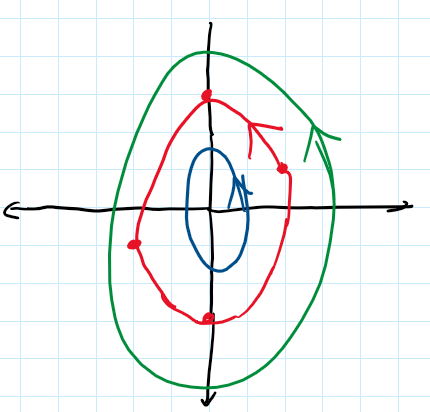
\includegraphics[height=1.5in]{Images/phaseportrait_1_n2_5_n1_sketch.png}}\hfill\hfill c)~$x = \frac{\sqrt{10}}{3}$
}

\begin{exercise}%\ansMark%
Find the general solution of the system
\begin{equation*}
{\vec{x}}' = \begin{bmatrix} 4 & 1 \\ -5 & 2 \end{bmatrix} \vec{x}
\end{equation*}
and sketch the phase portrait for this system.
\end{exercise}
\comboSol{%
}
{%
$\vec{x}(t) = C_1e^{3t} \left[\begin{smallmatrix} -\cos(2t) \\ \cos(2t) + 2\sin(2t) \end{smallmatrix}\right] + C_2e^{3t}\left[\begin{smallmatrix} -\sin(2t) \\ \sin(2t) - 2 \cos(2t) \end{smallmatrix}\right]$ \hfill\raisebox{-0.5\height}{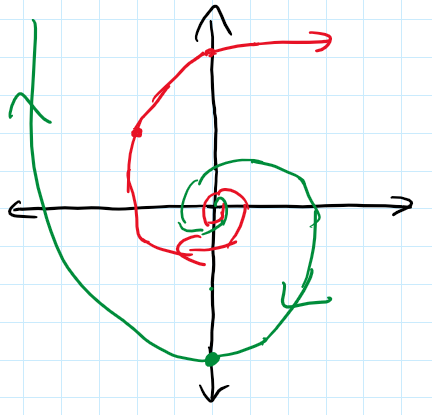
\includegraphics[height=1.5in]{Images/phaseportrait_4_1_n5_2_sketch.png}}\hfill\hfill
}


\begin{exercise}%\ansMark%
Find the general solution of the system
\begin{equation*}
{\vec{x}}' = \begin{bmatrix} 1 & 4 \\ -2 & -3 \end{bmatrix} \vec{x}
\end{equation*}
and sketch the phase portrait for this system.
\end{exercise}
\comboSol{%
}
{%
$\vec{x}(t) = C_1e^{-t}\left[\begin{smallmatrix} \cos(2t) - \sin(2t) \\ -\cos(2t) \end{smallmatrix}\right] + C_2e^{-t}\left[\begin{smallmatrix} \sin(2t) + \cos(2t) \\ -\sin(2t) \end{smallmatrix}\right]$ \hfill\raisebox{-0.5\height}{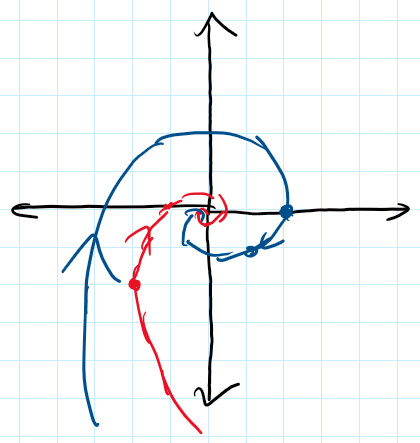
\includegraphics[height=1.5in]{Images/phaseportrait_1_4_n2_n3_sketch.png}}\hfill\hfill
}

\begin{exercise}%\ansMark%
Find the general solution of the system
\begin{equation*}
{\vec{x}}' = \begin{bmatrix} 2 & 0 & 3 \\ -6 & 2 & -9 \\ -3 & 0 & 2 \end{bmatrix} \vec{x}.
\end{equation*}
\end{exercise}
\comboSol{%
}
{%
$\vec{x}(t) = C_1\left[\begin{smallmatrix} 0 \\ 1 \\ 0 \end{smallmatrix}\right]e^{2t} + C_2e^{2t}\left[\begin{smallmatrix} \cos(3t) \\ -2\cos(3t) - 2\sin(3t)\\ -\sin(3t) \end{smallmatrix}\right] + C_3e^{2t}\left[\begin{smallmatrix} \sin(3t) \\ 2\cos(3t) - 3\sin(3t) \\ \cos(3t) \end{smallmatrix}\right]$
}

\begin{exercise}%\ansMark%
Find the general solution of the system
\begin{equation*}
{\vec{x}}' = \begin{bmatrix} -10 & -4 & 0 \\ 14 & 4 & 1 \\ 12 & 6 & -2 \end{bmatrix} \vec{x}.
\end{equation*}
\end{exercise}
\comboSol{%
}
{%
$\vec{x}(t) = C_1\left[\begin{smallmatrix} -1 \\ 2 \\ 2 \end{smallmatrix}\right]e^{-2t} + C_2e^{-3t} \left[\begin{smallmatrix} -4\cos(t) \\ 7\cos(t) - \sin(t) \\ 6\cos(t)  \end{smallmatrix}\right] + C_2e^{-3t}\left[\begin{smallmatrix} -4\sin(t) \\ 7\sin(t) + \cos(t) \\ 6\sin(t) \end{smallmatrix}\right]$
}

\begin{exercise}
Solve the initial value problem
\[ {\vec{x}}' = \begin{bmatrix} 3 & -1 \\ 4 & 3 \end{bmatrix} \vec{x} \qquad \vec{x}(0) = \begin{bmatrix} 2 \\ -1 \end{bmatrix}. \]
\end{exercise}
\comboSol{%
}
{%
$\vec{x}(t) = e^{3t} \left[\begin{smallmatrix}2\cos(2t) + \frac{1}{2}\sin(2t) \\ -\cos(2t) + 4\sin(2t) \end{smallmatrix}\right]$
}


\begin{exercise}
Solve the initial value problem
\[ {\vec{x}}' = \begin{bmatrix} -8 & -8 \\ 5 & 4 \end{bmatrix} \vec{x} \qquad \vec{x}(0) = \begin{bmatrix} 1 \\ 1 \end{bmatrix}. \]
\end{exercise}
\comboSol{%
}
{%
$\vec{x}(t) = e^{-2t}\left[\begin{smallmatrix} \cos(2t) - 7\sin(2t)\\ \cos(2t) + \frac{11}{2}\sin(2t) \end{smallmatrix}\right]$
}

\begin{exercise}
Solve the initial value problem
\[ {\vec{x}}' = \begin{bmatrix}-1 & 2 & -8 \\ 0 & 1 & -4 \\ 0 & 2 & -3 \end{bmatrix} \vec{x} \qquad \vec{x}(0) = \begin{bmatrix} 2 \\ 1 \\ -3 \end{bmatrix}. \]
\end{exercise}
\comboSol{%
}
{%
$\vec{x}(t) = e^{-t}\left[\begin{smallmatrix} -7 + 5\cos(2t) + 13\sin(2t) \\ \cos(2t) + 7\sin(2t) \\ -3\cos(2t) + 4\sin(2t) \end{smallmatrix}\right]$
}

\setcounter{exercise}{100}












